\chapter{Experiments}\label{chapter:experiment}

\section{Case studies}
Because the main work of this thesis is compare and evaluate performance between 
of algorithm, we just consider some simple case studies.
\paragraph{Dijkstra’s algorithm for mutual exclusion with a token}
The example illustrates a mutual exclusion algorithm \cite*{fribourg1997reachability} for agents forming a ring. 
They pass around a single token as a semaphore for a critical region.
\paragraph{Other mutual exclusion algorithms}
Additionally, we also consider the mutual exclusion algorithms of the standard bakery algorithm \cite*{chen2017learning}.
\paragraph{Dining philosophers}
Atomic
\paragraph{Cache coherence protocols}
When checking for cache coherence protocols, it's important to ensure that there aren't two different versions of the same data point present in the cache. 
In this regard, we only analyze the protocol MESI. 
We also examine different custom safety properties for each of these protocols.
The models are babse on \cite*{delzanno2000automatic}.
\paragraph{Leader election}
HERMAN
\paragraph{Token passing}
In conclusion, this thesis presents several examples that demonstrate token passing algorithms that we previously introduced 
in \autoref{chapter:preliminaries}.

\section{Dodo-cpp}
Dodo-cpp is a program that has three interpretations, namely trap, siphon, and flow. 
It runs for every system with four algorithms, which are $L^*$, $NL^*$, Kearns and Vazirani, Rivest-Schapire. 
After that, it plotted the graphs to compare the learned time 
of theses algorithms.

After running the algorithms, 
Dodo-cpp plots graphs to compare the time taken for each algorithm to learn. 
To make the data easier to analyze, the program uses the mathplot library \cite*{Hunter:2007} for graph plotting.


\section{Graphs}
The experiments in this thesis were running on x64 Ubuntu 22.04 system with 12th Gen Intel(R) Core(TM) i7-12700F processor
and 16GiB memory.

For all Figures, we use KV as an abbreviation for Kearns and Vazirani's algorithm and RS for Rivest-Schapire's algorithm.
All of the algorithms we used to learn produced the same results, regardless of their configuration and whether they could learn. 
However, the learning time for each algorithm varied. 
In the case of learning for a token-passing system using Trap and TrapSAT \footnote{\label{foot:sat}Use SAT-Sovler for the word problem.} interpretation and the "notoken" property,
\autoref{fig:trap_tokenpassing} shows that the inductive statements can be learned (marked with blue bars). 
We can also compare the learning time between the algorithms to determine which one is more effective.
\begin{figure}[h]
    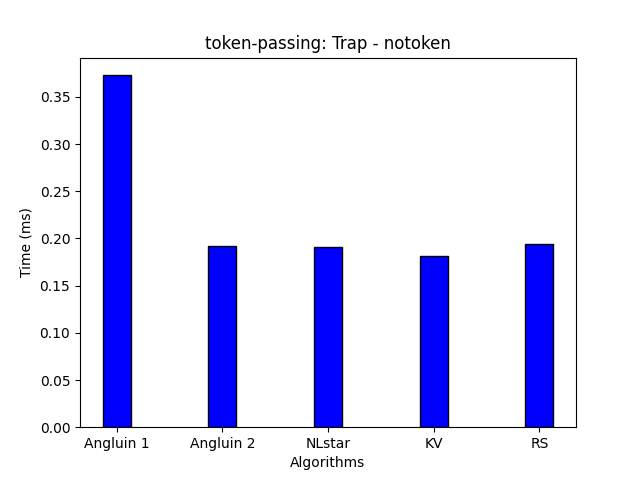
\includegraphics[scale=0.5]{figures/Trap_notoken.png}
    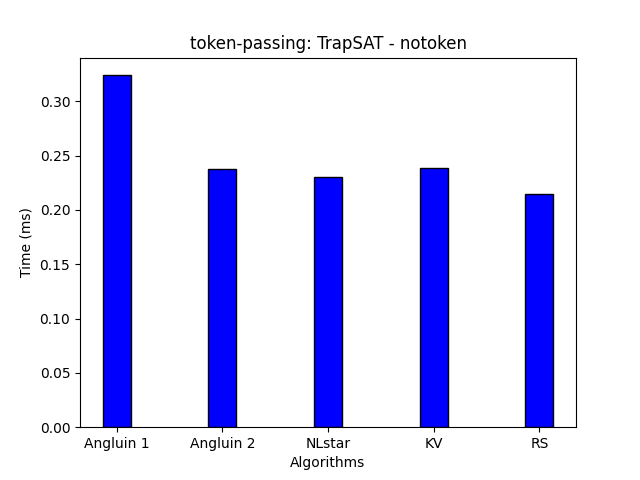
\includegraphics[scale=0.5]{figures/TrapSAT_notoken.png}
    \caption{\textit{Comparing the learning time of all algorithms; Result: success; Interpretation: Trap, TrapSAT; System: token-passing; property: notoken.}} 
    \label{fig:trap_tokenpassing}
\end{figure}

In \autoref{fig:siphon_tokenpassing}, we cannot learn using the Siphon and SiphonSAT\footnoteref{foot:sat} interpretation. We denote these cases with red bars.
\begin{figure}[h]
    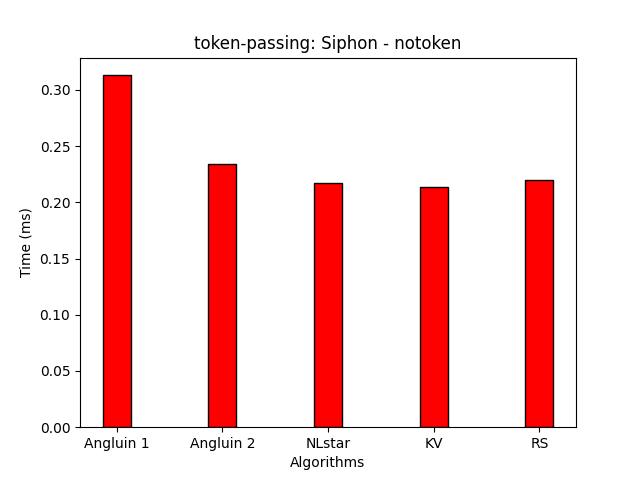
\includegraphics[scale=0.5]{figures/Siphon_notoken.png}
    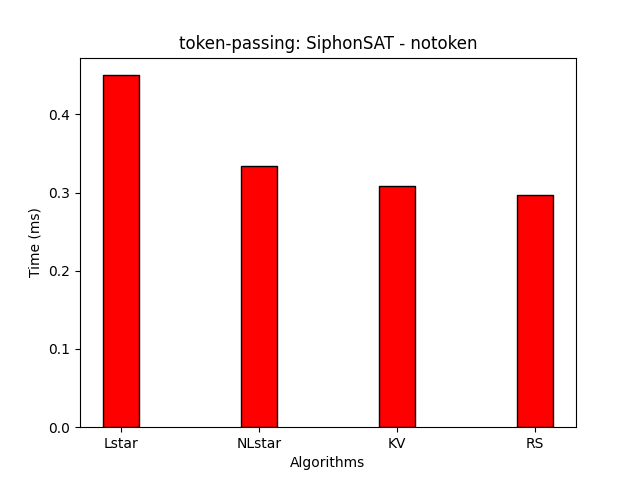
\includegraphics[scale=0.5]{figures/SiphonSAT_notoken.png}
    \caption{\textit{Comparing the learning time of all algorithms; Result: fail; Interpretation: Siphon, SiphonSAT; System: token-passing; property: notoken.}}
    \label{fig:siphon_tokenpassing}
\end{figure}

\section{Evaluating}

In \autoref{fig:average_membership}, we compare the number of memeber ship queries that are asked by each algorithm.
Because in our algorithm, we add the alphabet gradually and it causes membership queries
of all algorithm are the same.

we can not say for which algorithm is the best for all cases but at least we know in specifics configuration
which one is better.
\begin{figure}[h]
    \centering
    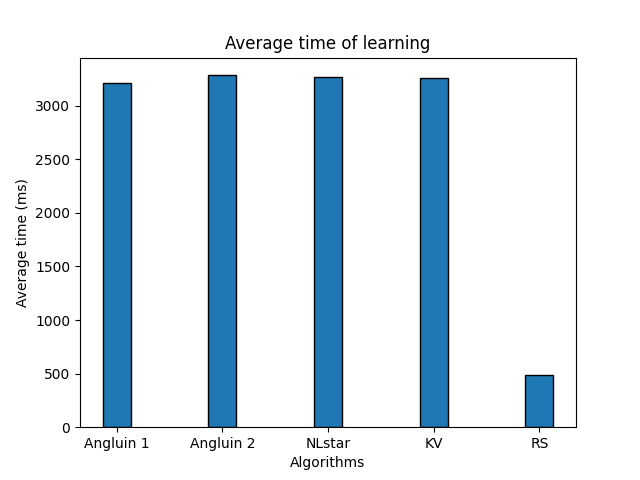
\includegraphics[scale=0.75]{figures/average_time.png}
    \caption{\textit{Comparing the average learning time of all algorithms.}}
    \label{fig:average_time}
\end{figure}

\begin{figure}[h]
    \centering
    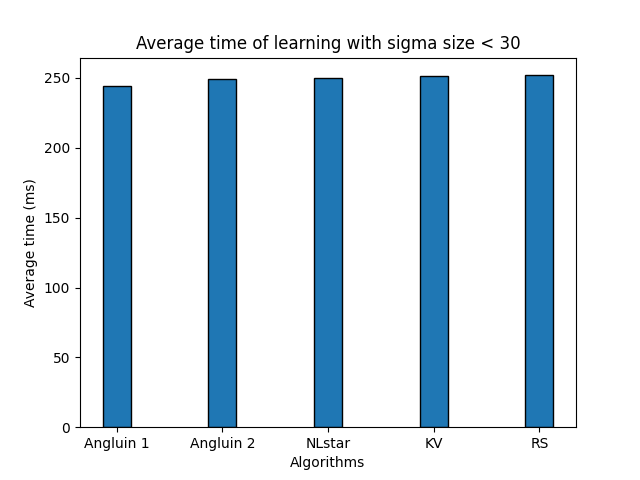
\includegraphics[scale=0.75]{figures/average_time2.png}
    \caption{\textit{Comparing the average learning time of all algorithms for all configurations with have $|\Sigma|$ < 30.}}
    \label{fig:average_time2}
\end{figure}

\begin{figure}[h]
    \centering
    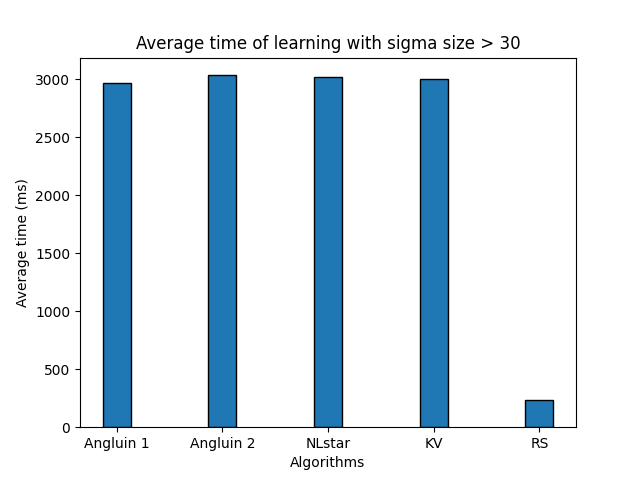
\includegraphics[scale=0.75]{figures/average_time3.png}
    \caption{\textit{Comparing the average learning time of all algorithms for all configurations with have $|\Sigma| \geq$  30.}}
    \label{fig:average_time3}
\end{figure}

\begin{figure}[h]
    \centering
    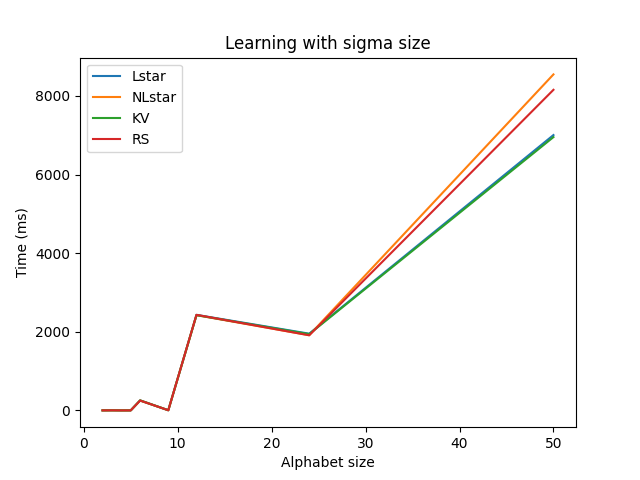
\includegraphics[scale=0.75]{figures/sigma_size.png}
    \caption{\textit{Comparing the average learning time of all algorithms corressponds to $|\Sigma|$.}}
    \label{fig:sigma_size}
\end{figure}

\begin{figure}[h]
    \centering
    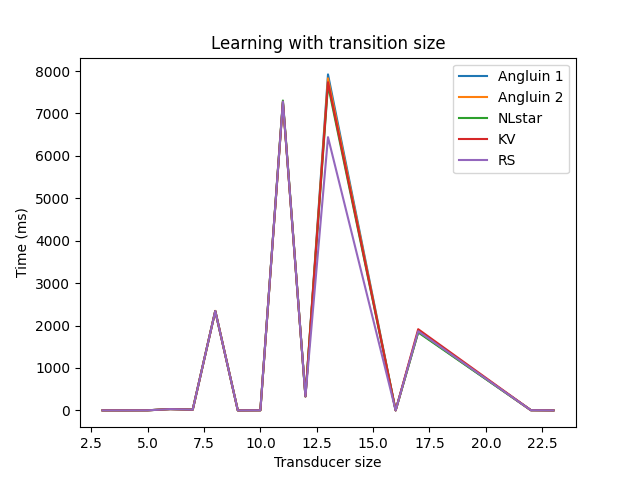
\includegraphics[scale=0.75]{figures/transition_size.png}
    \caption{\textit{Comparing the average learning time of all algorithms corressponds to transducer size.}}
    \label{fig:transition_size}
\end{figure}

\begin{figure}[h]
    \centering
    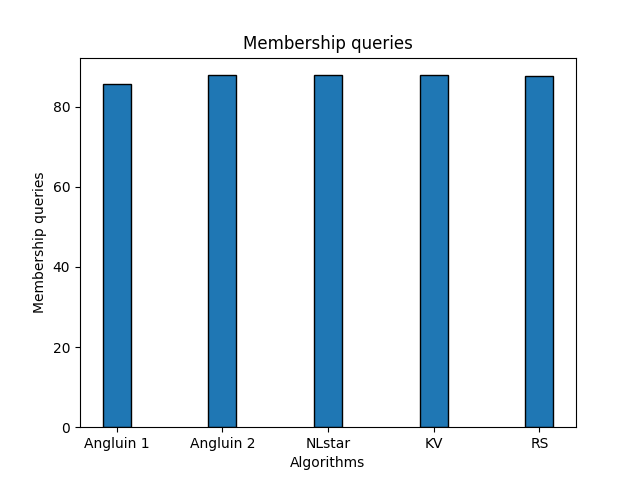
\includegraphics[scale=0.75]{figures/average_membership.png}
    \caption{\textit{Comparing the average membership queries of all algorithms.}}
    \label{fig:average_membership}
\end{figure}